In this experiment we used the example from \cite[Section 4.2.6]{jørgen2021}. The SRVT was not used in the original experiment, but the resulting optimization problem is the same. Thus, we considered a curve with SRV form \(q\) given by 
\begin{equation*}
    r(t) = \pi [-2 \sin(2\pi t), 4\cos(4\pi t)],
\end{equation*}
and its reparametrization \(q = \sqrt{\psi'}q \circ \psi\), where 
\begin{equation*}
    \psi(t) = \frac{\log(20t + 1)}{2 \log(21)} + \frac{\tanh(20(t - 0.5))}{4 \tanh(10)}.
\end{equation*}
The SRV form of the curves is shown in Figure \ref{fig:curve_1}. 

\begin{figure}[b]
    % \begin{subfigure}[b]{0.5\textwidth}\label{fig:curve_1_c_1}
    %     \centering
    %     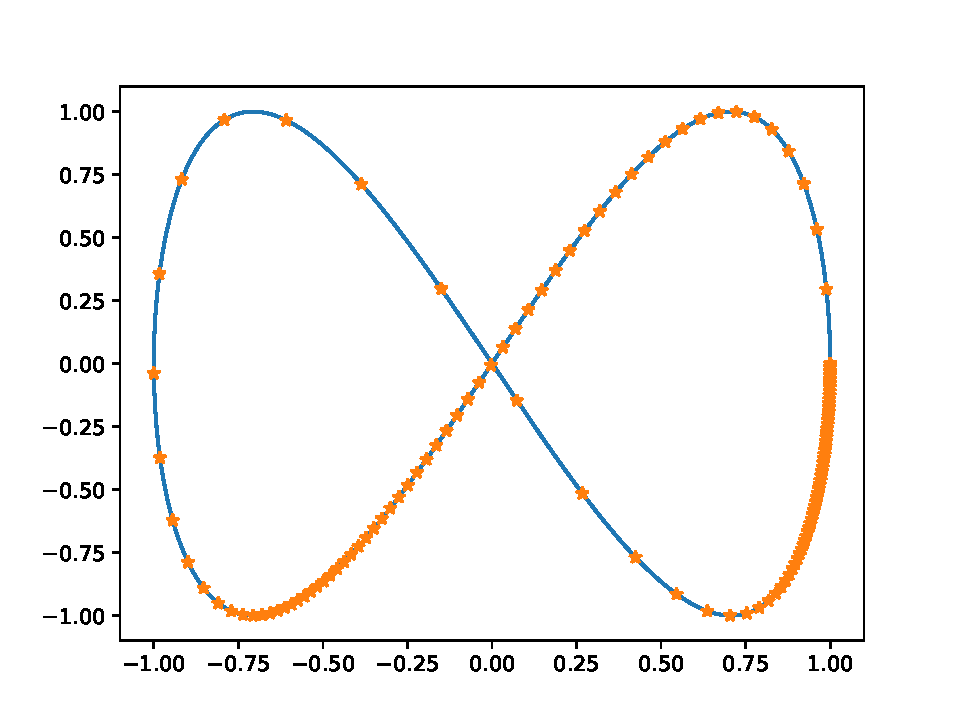
\includegraphics[width=\linewidth]{figures/curve_1/curve_c_1.pdf}
    %     \caption{\(c_1\)}
    % \end{subfigure}
    % \begin{subfigure}[b]{0.5\textwidth}\label{fig:curve_1_c_2}
    %     \centering
    %     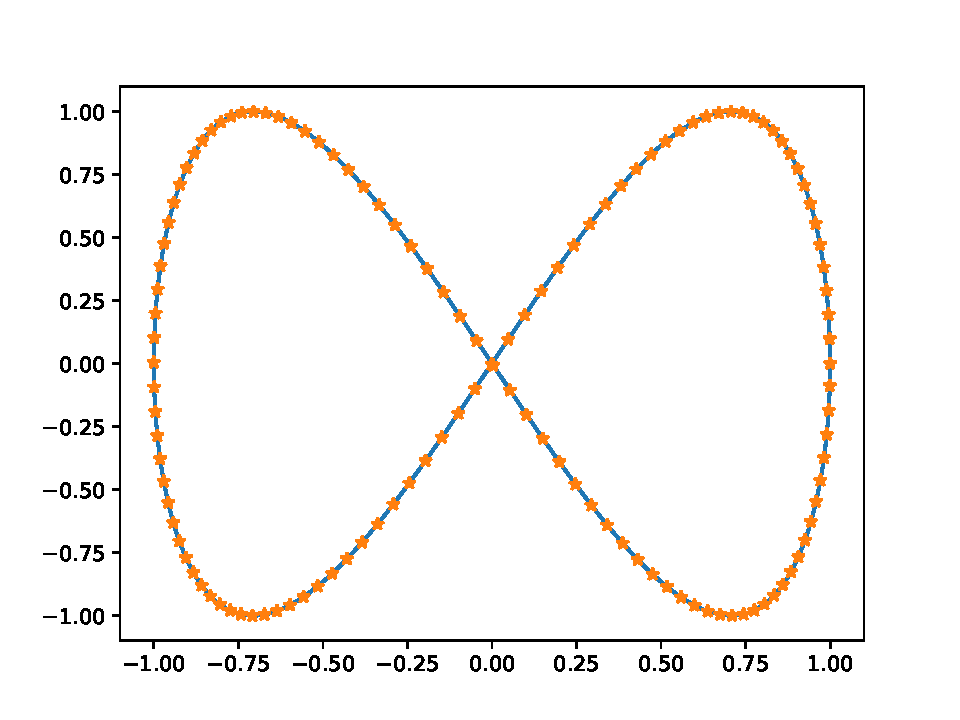
\includegraphics[width=\linewidth]{figures/curve_1/curve_c_2.pdf}
    %     \caption{\(c_2\)}
    % \end{subfigure}
    \begin{subfigure}[t]{0.5\textwidth}
        \centering
        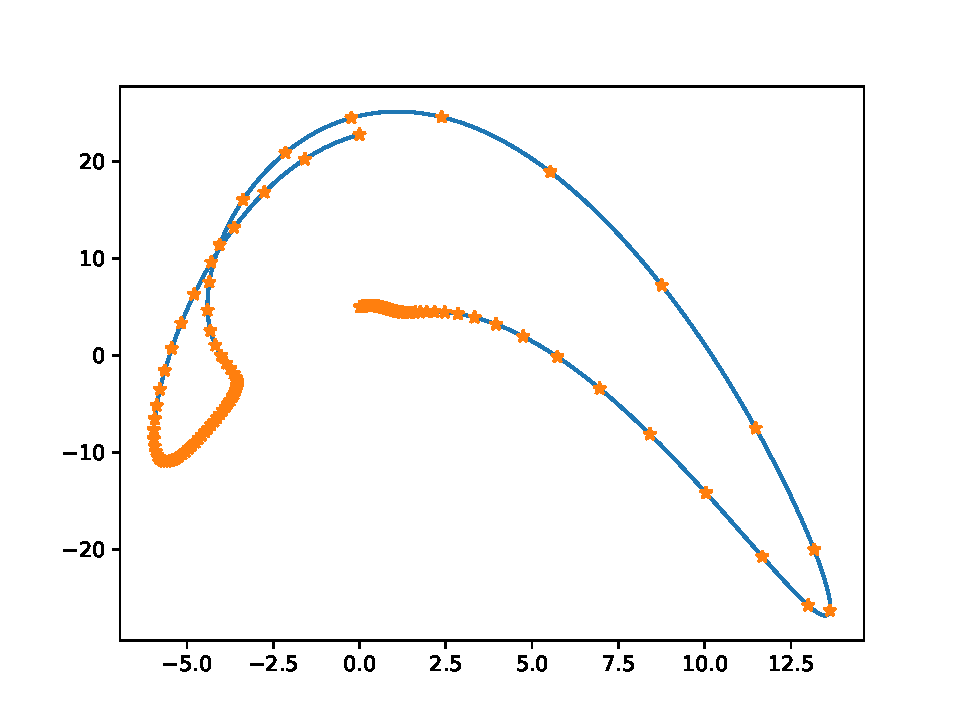
\includegraphics[width=\linewidth]{figures/curve_1/curve_q.pdf}
        \caption{\(q\)}\label{fig:curve_1_q}
    \end{subfigure}
    \begin{subfigure}[t]{0.5\textwidth}
        \centering
        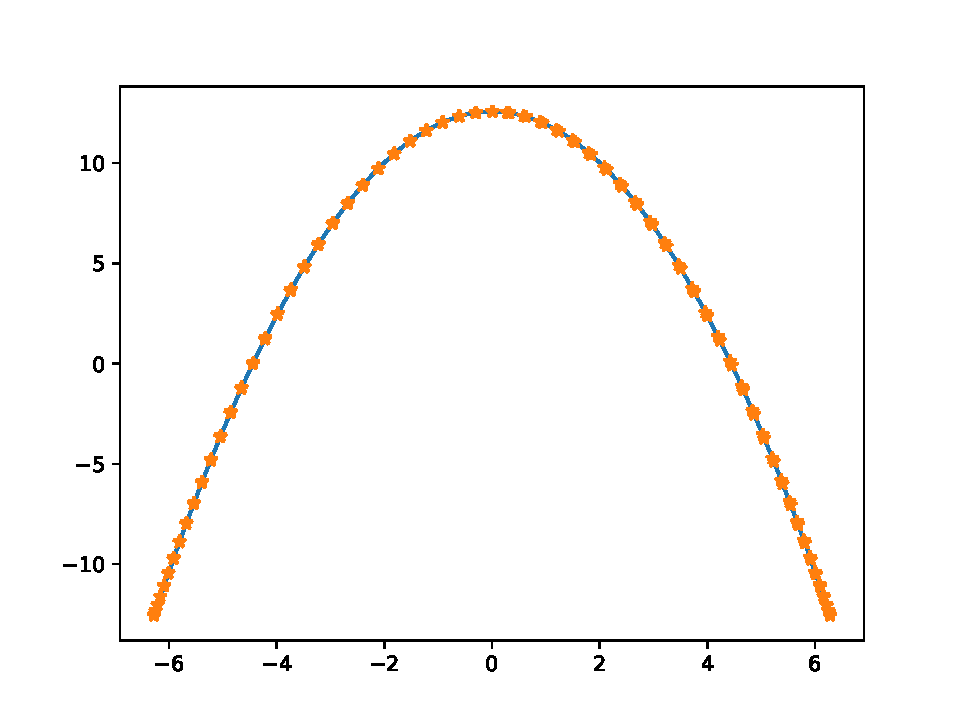
\includegraphics[width=\linewidth]{figures/curve_1/curve_r.pdf}
        \caption{\(r\)}\label{fig:curve_1_r}
    \end{subfigure}
    \caption{The trajectories of \(q\) and \(r\)}\label{fig:curve_1}
\end{figure}


\begin{figure}
    \begin{subfigure}[t]{0.5\textwidth}
        \centering
        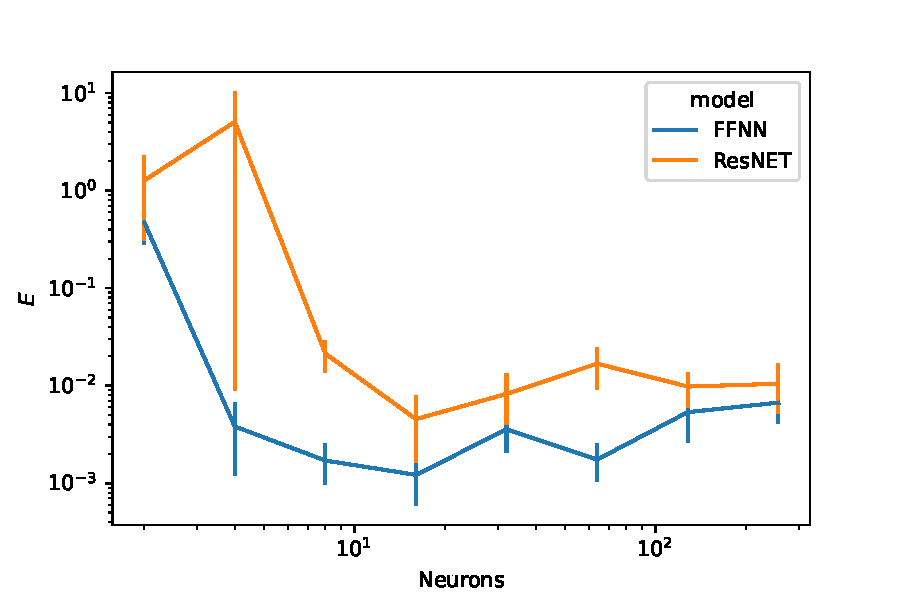
\includegraphics[width=\linewidth]{figures/curve_1/eks_5/neurons_error.pdf}
        \caption{The final cost \(E\) with the number of neurons in each hidden layer.} \label{fig:curve_1_neuron_error} \end{subfigure}
    \begin{subfigure}[t]{0.5\textwidth}
        \centering
        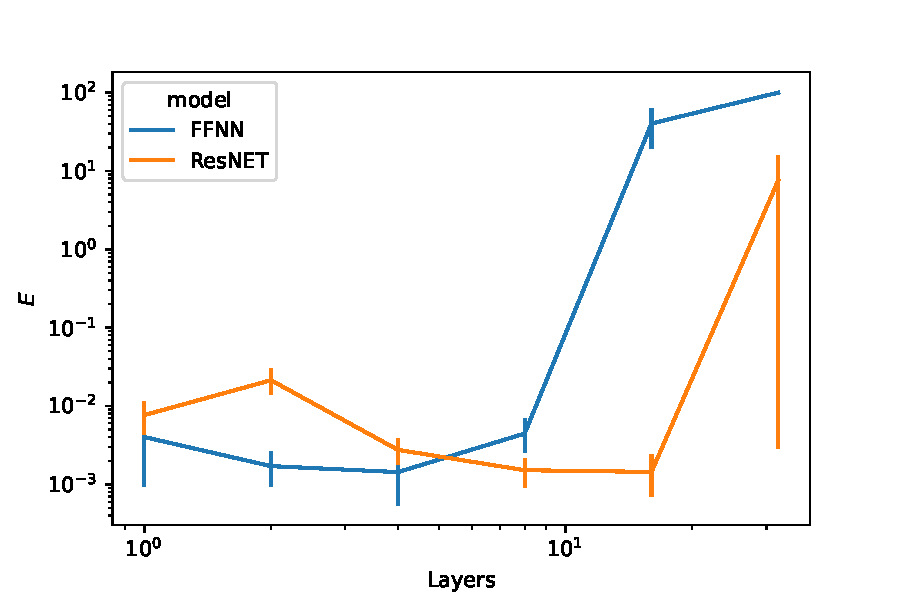
\includegraphics[width=\linewidth]{figures/curve_1/eks_5/layer_error.pdf}
        \caption{Final cost \(E\) with the number of hidden layers.} \label{fig:curve_1_layer_error}
    \end{subfigure}
    \caption{Result of ensemble training with different number of neurons and hidden layers. In Figure \ref{fig:curve_1_neuron_error} the number of layers was fixed at 2. In Figure \ref{fig:curve_1_layer_error} the number of neurons is fixed at 8 per hidden layer. The error bars denote a 80\% confidence interval found by bootstrapping.} \label{fig:curve_1_parmas_eks}
\end{figure}

\begin{figure}[b]
    \begin{subfigure}[t]{0.5\textwidth}
        \centering
        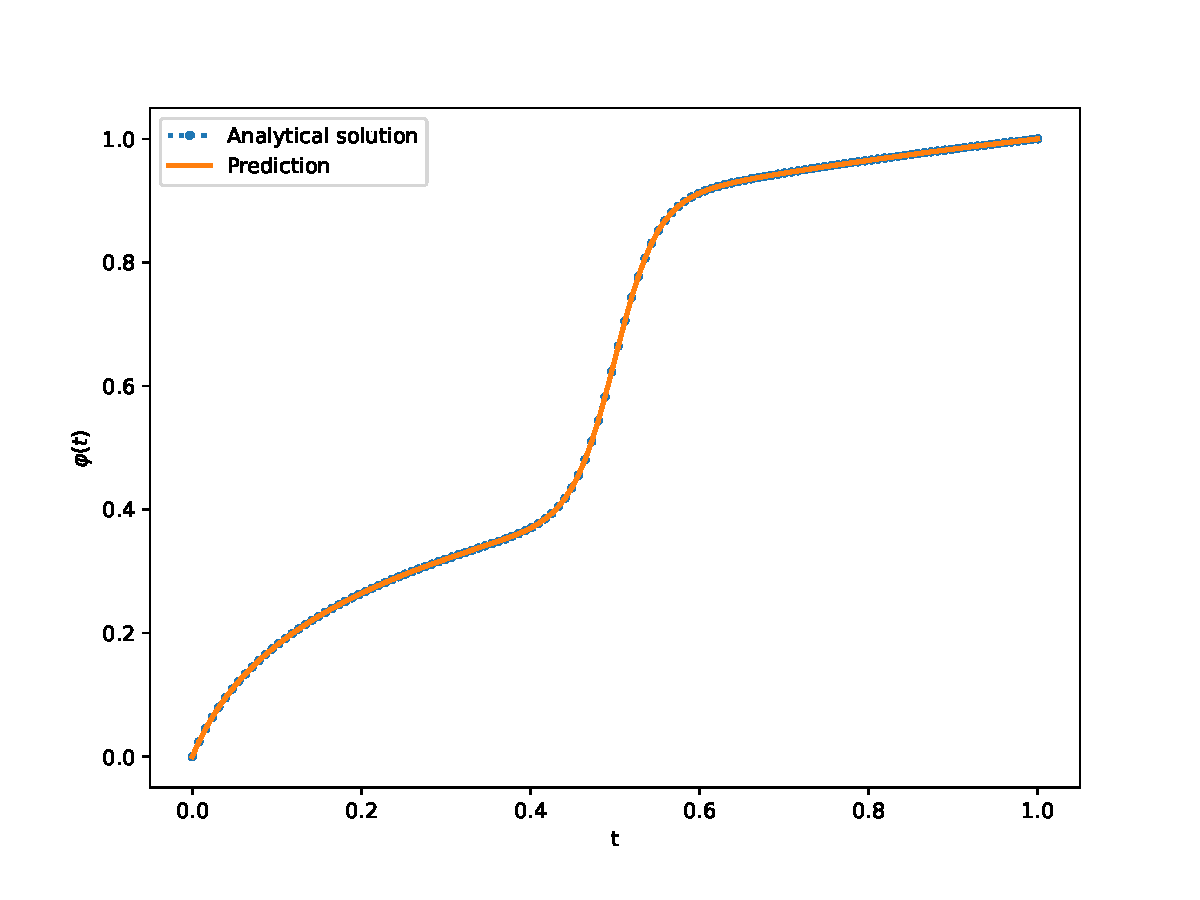
\includegraphics[width=\linewidth]{figures/curve_1/eks_5/plot_2_0.pdf}
        \caption{The approximate optimal reparametrization and the analytical solution.}\label{fig:curve_1_solution}
    \end{subfigure}
    \begin{subfigure}[t]{0.5\textwidth}
        \centering
        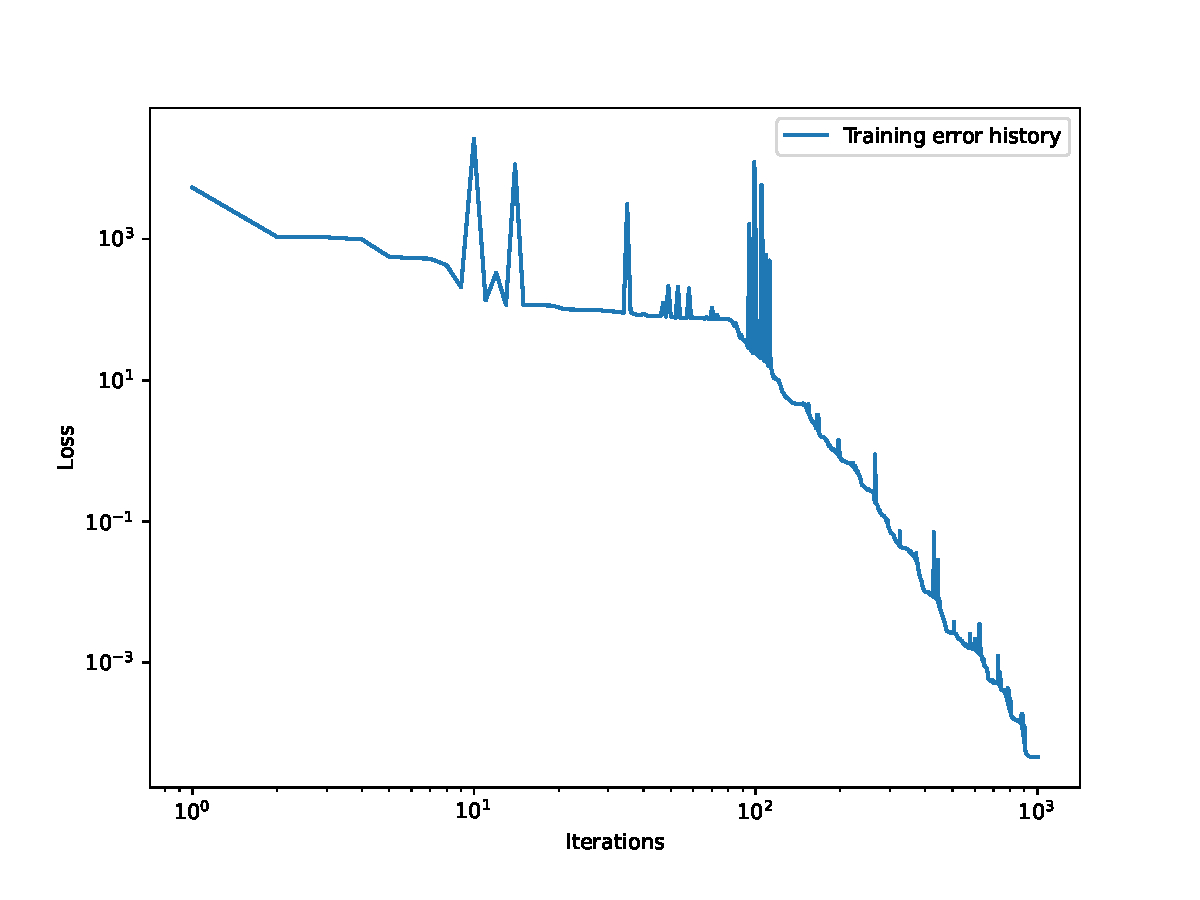
\includegraphics[width=\linewidth]{figures/curve_1/eks_5/history_plot_2.pdf}
        \caption{The cost function \(\mathcal{J}(\theta)\) with each iteration.}\label{fig:curve_1_history}
    \end{subfigure}
    \caption{Result of one optimization procedure with the corresponding loss history.}\label{fig:curve_1_example}
\end{figure}


We performed ensemble training with different network structures, lengths, and widths to test how our method performs on the problem. An overview of the result is shown in Figure \ref{fig:curve_1_parmas_eks}. Moreover, the resulting optimal reparametrization of the first training procedure can be seen in Figure \ref{fig:curve_1_example}. One possible observation is that a ResNet structure permits the training of deeper neural networks better than fully connected feedforward networks.

Reparametrization by neural networks was also compared to deep reparametrization. The comparison was made with respect to the cost function \(\hat E\), as defined in \eqref{eq:discretized_cost}, and is shown in Table \ref{tab:comare_res_palais}. We see that deep reparametrization outperforms our method significantly for this problem. Moreover, deep reparametrization produced the same solution for each training. This is not the case for reparametrization by neural networks since the initial condition \(\theta_0\) is random.
\begin{table}[b]
    \centering
    \begin{tabular}{lrl}
        \toprule
        \(\hat{E} \) & Degrees of freedom & Model         \\
        \midrule
        0.013143     & 34                 & ResNet        \\
        0.002253     & 9391               & ResNet        \\
        0.004567     & 30                 & Palais Layers \\
        0.000002     & 10000              & Palais Layers \\
        \bottomrule
    \end{tabular}
    \caption{Comparison of the performance of reparametrization by residual neural network and deep reparametrization. Each experiment is the average of 10 optimisation procedures. Deep reparametrization was performed using Palais Layers.}\label{tab:comare_res_palais}
\end{table}
